\section{Experimental procedure}
In this experiment, we set up two detectors with equidistant from the source (5cm apart). We adjusted fast and slow signals circuits and both of them combined in to a Universal Counter(UC) through a gate and delay($G^{2}-D^{2}$). Two CFD are connected to filter out zero crossing in fast signal circuit and two amplifiers are connected in slow signal circuit. We used three delays, two in slow signal circuit and one between CFD2 and FC. A timer connected with all counters to fixed the counting time. The figure ~\ref{fig:CCuit} shows a schematic of the set and the tasks we did on this experiment are described in the following.

\begin{figure}[ht]
	\centering
	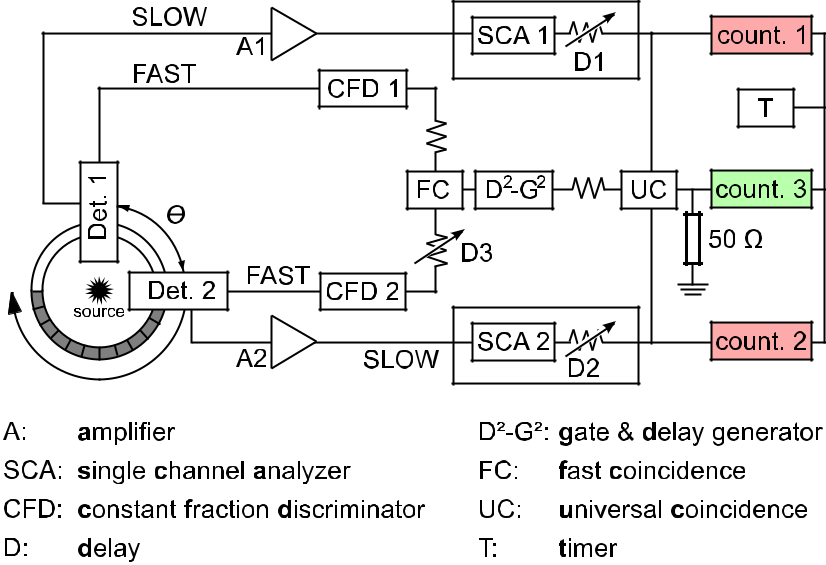
\includegraphics[width=0.8\linewidth]{./figs/CirCuit.png}
	\caption{Set up of fast and slow coincidence circuit~\cite{descr}.}%
	\label{fig:CCuit}
\end{figure}
\subsection{Adjusting the gain of the Amplifier}
First, we adjusted the gain of both amplifiers  ($A_{1}$ and  $A_{2}$) during the set up of the experiment. The amplifiers output is linear up to $V_{max}=9$ V. We visualized the signal, with the help of Oscilloscope, and set the amplification of amplifiers  to obtain a signal with maximum around 9 V. Here we took gain of the amplifier as much as possible because larger signals are easier to process. We had been keeping in mind that the upper limit of the gain is used in the set up which is given by the signal range of the electronics. Figure ~\ref{fig:Amplified} shows the amplified signal from the Amplifier1.

\begin{figure}[ht]
	\centering
	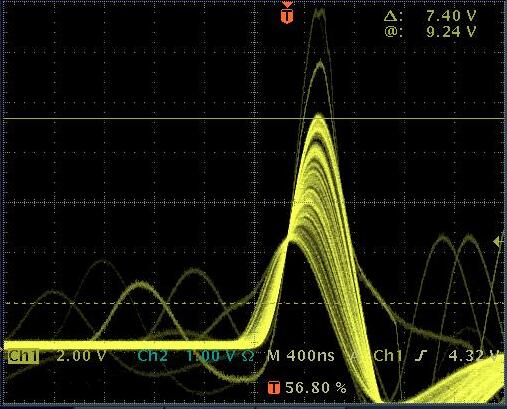
\includegraphics[width=0.8\linewidth]{./figs/Amplifier.jpg}
	\caption{Amplified Signal Output from the Detector. we set the amplification of amplifiers to obtain a signal with maximum at around 9 V.}%
	\label{fig:Amplified}
\end{figure}
\newpage
\subsection{Adjusting of the CFD}
CFD has a threshold-discriminator which help to filter out zero crossing that belongs to electronic noise and not to a true scintillation signal ~\cite{descer}. Performing a threshold scan allows to search out the right compromise. For that, CFD has restriction upon the minimum and maximum signals and it can manage two signals of same amplitude with different risetimes.  So, we have adjusted this threshold of CFD to detect only true signals not the background noise signals. In that step, We connected the negative outputs of the both CFDs to the counters and measured the count rates with and without source installed. Also, We connected a delay $ D_{3} $ between CFD2 and the Fast Coincidence(FC) to correct the delay within the resolving time. To appropriate gate duration, we calculated $\Delta N \approx \sqrt{N}$. Figure ~\ref{fig:Cfd1} and ~\ref{fig:Cfd2}, respectively, shows the CDF count rate with and without inserting source.

\begin{figure}[ht]
	\centering
	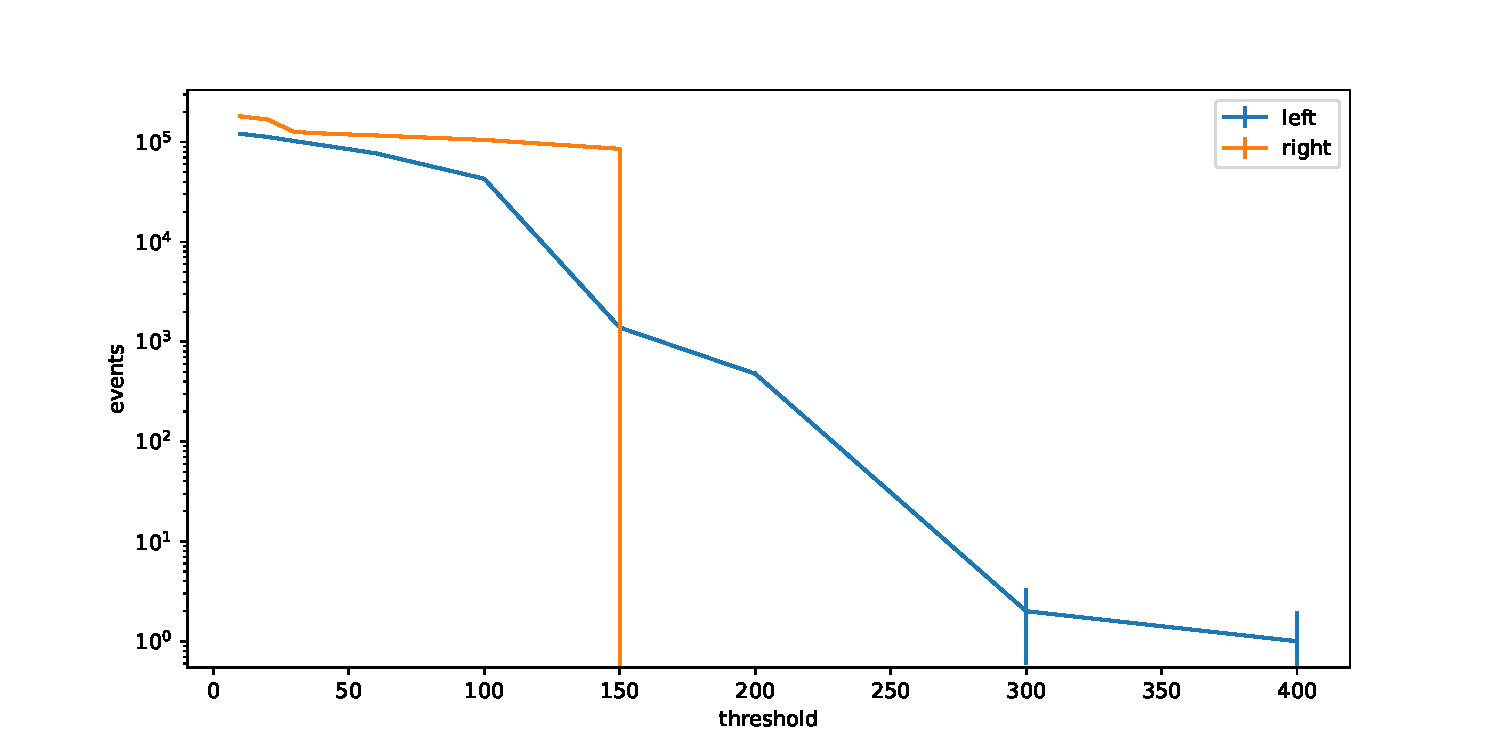
\includegraphics[width=0.8\linewidth]{./figs/cfd.pdf}
	\caption{CFD count rate with inserting source. Here threshold limit is [150-400]. }%
	\label{fig:Cfd1}
\end{figure}

\begin{figure}[ht]
	\centering
	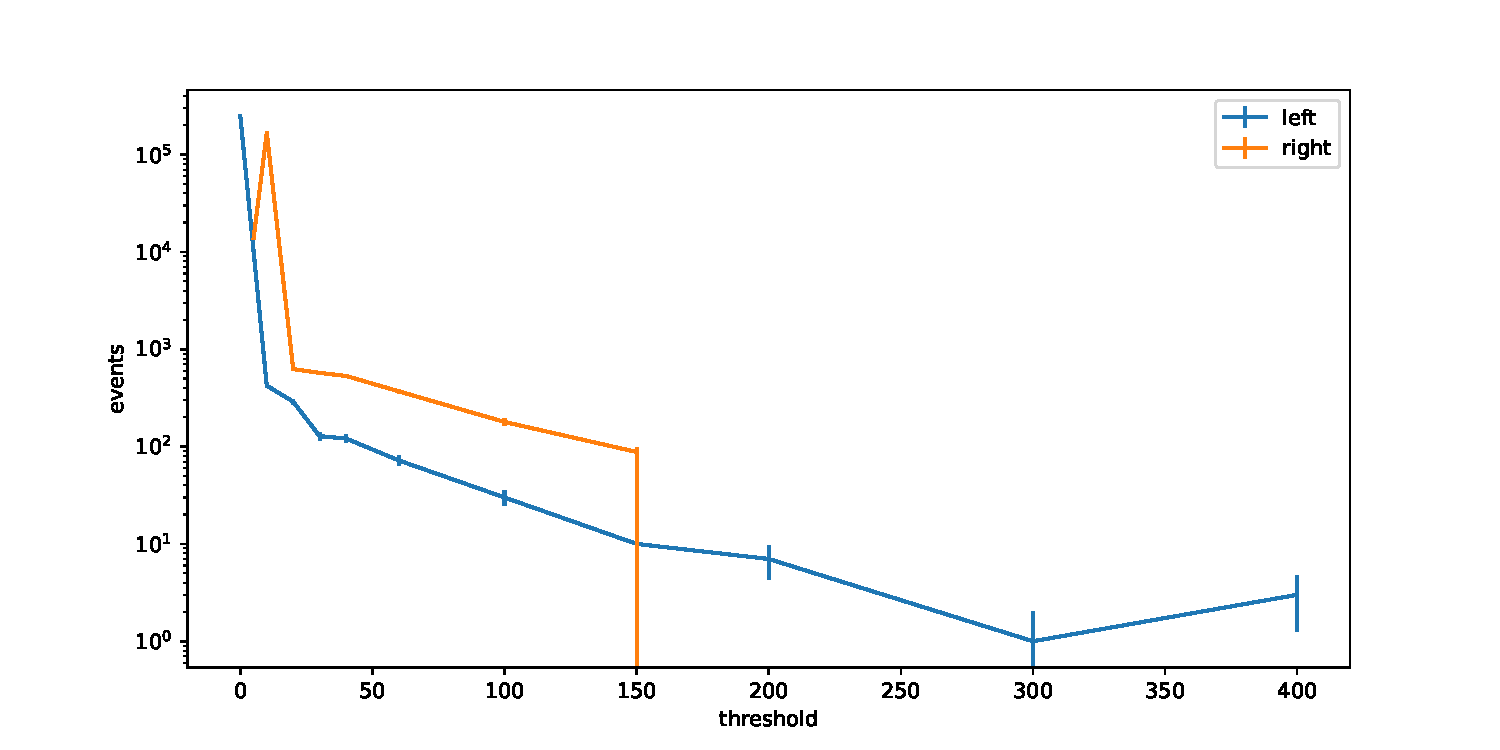
\includegraphics[width=0.8\linewidth]{./figs/cfd2.pdf}
	\caption{CFD count rate without inserting source. Here threshold limit is [150-400].}%
	\label{fig:Cfd2}
\end{figure}

\subsection{Setting up the Fast Coincidence}
In this step, we visualized the coincidence of incoming signals from two CFDs with the help of oscilloscope and then determined the proper delay. For that, we connected the negative outputs of both CFDs to the oscilloscope and triggered on the first channel signals. Then, on the second channel, true coincidence pulses are  appeared. The random time appearing events are uncorrelated. we Inserted a fixed delay into the fast branches and a variable delay into the other one set up with resolving time, so real coincidence restricted. For that, we inserted the fixed delay in between CFD1 and FC and a variable delay in between CFD2 and FC as shown in figure ~\ref{fig:CCuit}. Then, we Connected the outputs of the CFDs to the fast coincidence unit to measure the count rate for different delay settings of the variable delay unit and we picked the resolving time 25 ns. A  gate and delay $ G^{2}-D^{2} $connected between FC and UC, where both slow and fast signal inputs are connected. In this step, we adjusted the slow signal circuit for matching the pulses height and fast signal circuit for timing of the pulses.


\subsection{Setting up the Slow Coincidence}

Here, one hand,  we connected the output from the fast coincidence unit to a gate and delay ($ D^{2}-G^{2} $) generator module to adjust the timing. Other hand, the delay of both SCAs can be adjusted. Then, the output from ($ D^{2}-G^{2} $) inserted to the first channel and positive output from SCA1 and SCA2 on after another to the second channel of the oscilloscope. We need to align the leading edges of the signal which are align the timing of these three input signals with the help of oscilloscope. Afterward, we adjusted the delays in both SCAs and ($ D^{2}-G^{2} $). In figure ~\ref{fig:slow} we can see the peaks from SCAs are inside the peak of the FC unit.


\begin{figure}[ht]
	\centering
	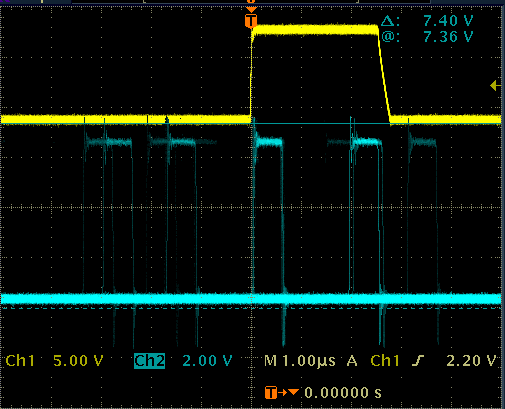
\includegraphics[width=0.8\linewidth]{./figs/slow.png}
	\caption{The timing alignment of signals from FC and two SCAs.}%
	\label{fig:slow}
\end{figure}


\subsection{Calibrating the Signal Channel Analyzer}
The SCAs are used to select the whole energy deposited events of gamma rays from our source in the corresponding detector. 
In this step, we performed the energy calibration and recorded the energy-spectrum by using SCAs which are produces an output logic only when peak amplitude of the input signals are within threshold limit. So, For that, we set the SCAs to their window mode which is only set by second knob. Later we keep the constant obtained window size for all measured points for normalization. The window-width play important role on output. We have to  marked out all structures of energy spectrum in the selective energy range, so we started with 10,...,20 window-width. we increased the window size when energy appeared everywhere the same count rates; however, we try to decrease the window size as much as possible. The second peak on the right counter was not appear so we changed the amplification setting. Figures ~\ref{fig:sca1} and ~\ref{fig:sca2} shows the energy spectrum of $ ^{60}Co$-decay obtained by SCA1 and SCA2 respectively.


\begin{figure}[ht]
	\centering
	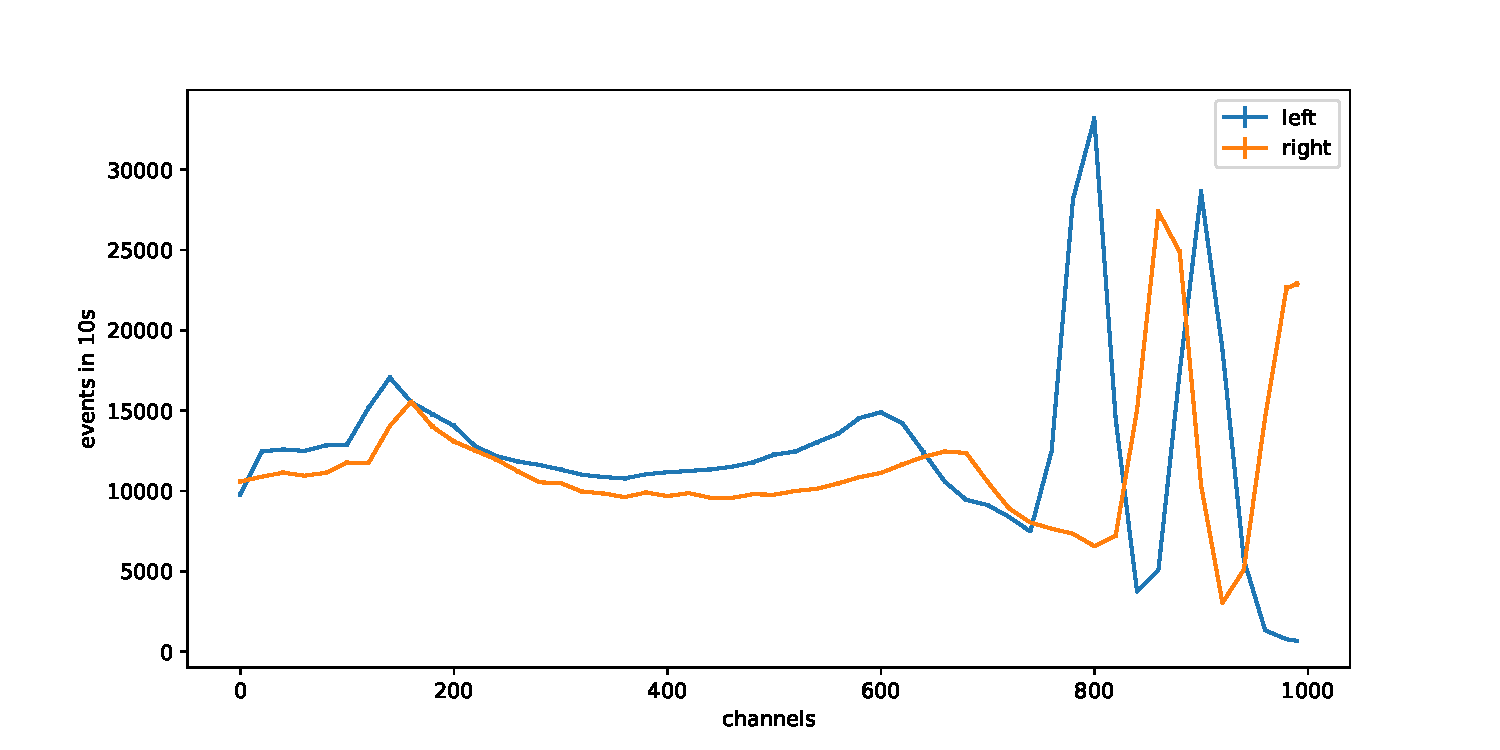
\includegraphics[width=0.8\linewidth]{./figs/sca.pdf}
	\caption{The energy spectra of SCA1. Here two peaks are in the range of [750-1000].}%
	\label{fig:sca1}
\end{figure}

\begin{figure}[ht]
	\centering
	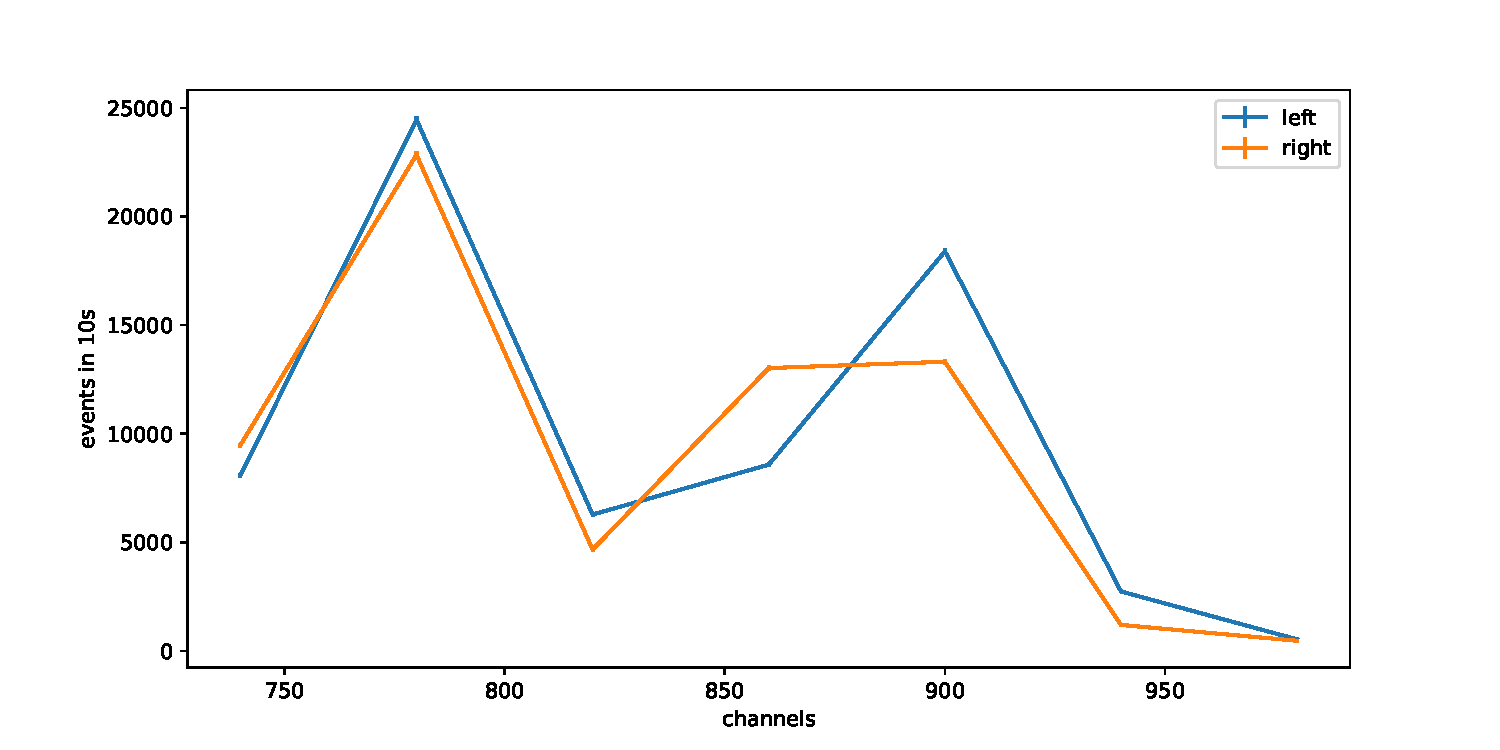
\includegraphics[width=0.8\linewidth]{./figs/sca2.pdf}
	\caption{The energy spectra of SCA2. Here two peaks are in the range of [750-950].}%
	\label{fig:sca2}
\end{figure}

\newpage
\subsection{Main Measurement}
After adjusting all the involving apparatus in the experiment, we stated to perform the main measurement of the experiment. we used two detectors, one of them is fixed and another is movable, place at equidistant (5cm) apart from the $ ^{60}Co$ source and  $180^{\circ} $ angular separation and we adjusted the SCA windows to cover both photo peaks. Then we measured the count rates for different angles between these two detectors. We had taken more than twenty measurement with angular range of $5^{\circ}$ some of them with $10^{\circ}$ few were randomly. We got precise data on some positions. Specially three measurements: first one to generate the idea of the angular correlation, middle one to find out the correlation coefficient and third one to get an idea of the stability of set up. Then, we repeated the measurement on different positions.

\begin{figure}[ht]
	\centering
	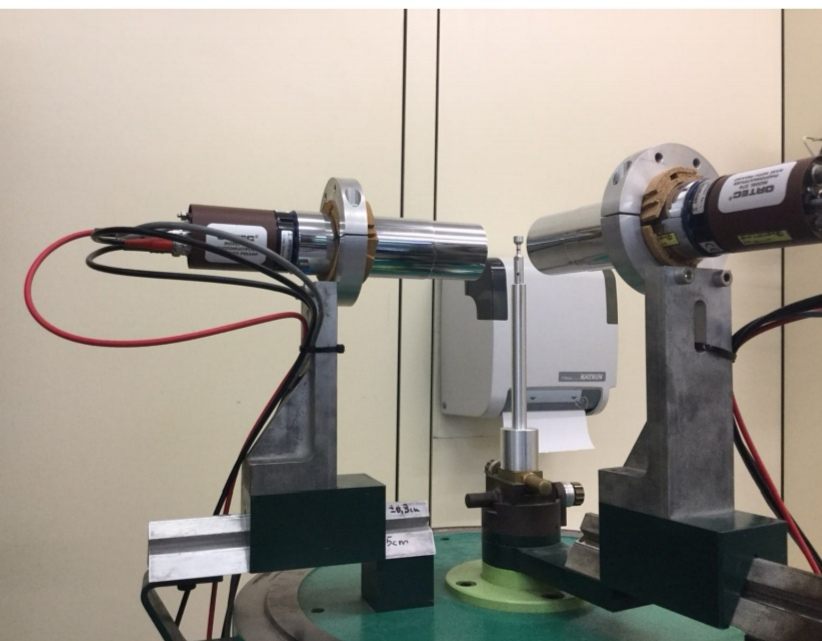
\includegraphics[width=0.8\linewidth]{./figs/detectors.jpg}
	\caption{Set up of two detectors where one is fixed and another one is movable to rotate at a fixed radial distance from the fixed detector.}%
	\label{fig:detect}
\end{figure}


